\documentclass[10pt,a4paper]{article}

\usepackage[utf8]{inputenc}


\usepackage{algpseudocode}
\usepackage{algorithmicx}
\usepackage{amsfonts}
\usepackage{amsmath}
\usepackage{amssymb}
\usepackage[spanish]{babel}
\usepackage[style=nature,intitle=true,sorting=none]{biblatex}
\usepackage{csquotes}
\usepackage{dsfont}
\usepackage{enumitem}
\usepackage{fancyhdr}
\usepackage{geometry}
\usepackage{graphicx}
\usepackage[hidelinks]{hyperref}
\usepackage{ifthen}
\usepackage[utf8]{inputenc}
\usepackage{multicol}
\usepackage{titling}
\usepackage{xcolor}
\usepackage{wrapfig}


\title{Organización del Computador II}
\author{Gianfranco Zamboni}

%%%% CONFIGURACIONES %%%%

%% La coma de los reales es un punto
\decimalpoint

%%% Tamaño de pagina
%\geometry{
%	includeheadfoot,
%	left=2.54cm,
%	bottom=1cm,
%	top=1cm,
%	right=2.54cm
%}

%\stul{0.1cm}{0.2ex}

%% HEADER Y FOOTER
\pagestyle{fancy}

\fancyhf{}

\fancyhead[LO]{\rightmark} % \thesection\ 
\fancyhead[RO]{\small{\thetitle}}
\fancyfoot[CO]{\thepage}
\renewcommand{\headrulewidth}{0.5pt}
\renewcommand{\footrulewidth}{0.5pt}
\setlength{\headsep}{1cm}
\setlength{\headheight}{13.07225pt}

\renewcommand{\baselinestretch}{1.2}  % line spacing

%% Links en indice 
\hypersetup{
	linktoc=all,     %set to all if you want both sections and subsections linked
	linkcolor=blue,  %choose some color if you want links to stand out
}

\newcommand{\red}[1]{{\color{red}#1}}  			% Rojo, duh (?)
\begin{document}
	\maketitle
	\tableofcontents
	\newpage

\section{Introducción}

La \textbf{arquitectura de computadoras} es la ciencia y arte de diseñar, seleccionar e interconectar hardware y diseñar las interfaces hardware/software para crear un sistema computacional que poosea los requerimientos funcionales, de perfomance, consumo (de energía) y de costo (económico) adecuados para realizar determinadas tareas.

\begin{wrapfigure}{r}{0.5\textwidth}
	\centering
	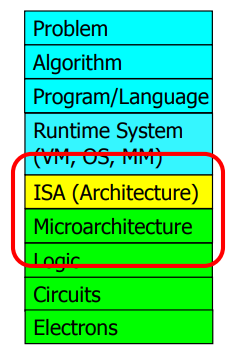
\includegraphics[width=0.25\textwidth]{imagenes/arquitectura}
	\caption{figure}{La computadora definida en niveles de abstracción}
	\label{fig:arquitectura}
\end{wrapfigure}

Estas tareas son problemas que pasaron por varias transformaciones (desde su descripción en un lenguaje natural hasta convertirse en un programa) y deben ser ejecutadas por una computadora. La tarea del arquitecto consiste en diseñar el \textbf{Instruction Set Architecture} (ISA), un conjunto de instrucciones que usarán los programas compilados para decir al micropocesador que hacer. El ISA es implementado por un conjunto de estructuras de hardware conocidas como la \textbf{microarquitectura} del procesador.

El ISA y la microarquitectura sientan las bases para el diseño del procesador y, como se dijo anteriormente, un buen diseño debe tener en cuenta los objetivos de sus usuarios y conseguir el balance adecuado de los factores mencionados para llevarlos a cabo de la manera más optima posible. Habrá casos en los que daremos prioridad a un subconjunto de ellos en detrimento de otros (por ejemplo, podriamos elegir mejorar perfomance y aumentar el costo, o quitar performance para mejorar el consumo energético).

\subsection{Componentes del ISA}
El ISA es la especificación completa de la interfaz entre los programas y el hardware que debe llevar a cabo las operaciones. El ISA especifíca:

\subsubsection{Regitros}
\begin{itemize}
	\item Los \textbf{registros},  celdas de memoria dentro dentro del cpu que son usados para almacenar temporalmente lo valores necesarios para ejecutar una instrucción. Estos registros son visibles al programa y se clasifican según su uso: Acumuladores, De dirección ó De Proposito General.
	\item Los mecanismos usados por la computadora para saber donde están almacenados los datos(\textbf{Espacio de memoria}), 
	\item La cantidad de bloques univocamente distinguibles en memoria y el tamaño de cada uno de estos bloques (\textbf{Direccionamiento})
	\item  Un conjunto de instrucciones  que pueden ser llevadas a cabo por la computadora. Cada instrucción está compuesta por su \textbf{opcode} (que se espera que la computadora haga) y sus \textbf{operandos} (a que datos debe hacerlo). En una ISA, podremos encontrar tres tipos de instrucciones:
	\begin{itemize}
		\item De \textbf{Operacion}: Procesan datos
		\item De \textbf{trasnporte de datos}: Transportan información entre la memoria, los registros y los dispositivos de entrada salida.
		\item De \textbf{control}: Modifican la secuencia de instrucciones a ser ejecutada, es decir permiten ejecutar instrucciones que no están almacenadas en el proximo bloque de memoria.
	\end{itemize}
	
	Depéndiendo que valores puedan modificar las instrucciones de operación, podremos clasificar las arquitecturas en \textbf{Arquitecturas Load/Store} (solo pueden operar en registros) o \textbf{Arquitecturas memory/memory} (se pueden modificar los valores directamente en memoria)
	\item los \textbf{Tipos de datos}, es decir que representación deben tener ciertos valores para que puedan ser interpretados por la microarquitectura
	\item Las formas en las que un operando puede ser accedido (\textbf{modos de direccionamiento}). Pueden ser:
	\begin{itemize}
		\item \textbf{Inmediato:} El operando está incluido en la instrucción.
		\item \textbf{Directo o absoluto:} El operando es la dirección de memoria donde se encuentra el valor a ser utilizado.
		\item \textbf{Indirecto:} El operando es una dirección de memoria, donde se encuentra la dirección de memoria en la que está almacenado el valor deseado.
		\item \textbf{De desplazamiento:} La instrucción toma como operandos una dirección de memoria que se toma como \textbf{base} y un \textbf{offset}, que es un número que indica cuanto hay que desplazar la base para encontrar el valor deseado, es decir $dir = base + offset$
		\item \textbf{Indexado:} Lo mismo que el anterior, pero con el \textit{offset} guardado en un registro.
		\item \textbf{De Memoria Indirecta:} El operando es un registro en el que se encuentra guardada la dirección de memoria indirecta.
	\end{itemize}
	\item Como comunicarse con los dispositivos de entrada/salida (\textbf{I/O Interface}), puede ser por medio de instrucciones especiales o mapeos de ciertas regiones memoria para esos dispositivos.
	\item Quien puede y quien no puede ejecutar certas instrucciones (\textbf{Modos de privilegios})
	\item Qué debe suceder si una instrucción falla o cuando un dispositivo necesita usar el microprocesador (\textbf{Manejo de excepciones e interrupciones})
	\item Si soporta o no el uso de \textbf{memoria virtual}, es decir, si cada programa tiene la ilusión de estar un espacio de memoria secuencial cuando en realidad el sistema operativo realiza el manejo de la memoria principal
\end{itemize}

\subsubsection{Arquitectura de Von Neumann}\label{Intro::ISA::Von_Neuman}
Como se vió en Organización del computador I, las mayoría de las ISA usadas actualmente usan el modelo de Von Neumann. Este un ciclo de cinco etapas: 

\begin{enumerate}
	\item \textbf{Fecth:} Se utiliza un \textbf{program counter} que indica donde está almacenada la proxima instrucción a ser ejecutada.
	\item \textbf{Decode:} Se decodifica la instrucción fetcheada y se consiguen los operandos (literales y registros) correspondientes.
	\item \textbf{Execute:} En esta etapa se busca en memoria los datos requeridos (si es necesario) y se procesa los datos acorde a la instruccióny se almacenan sus resultados en el lugar correspondiente.
\end{enumerate}

\begin{figure}[h]
	\centering
	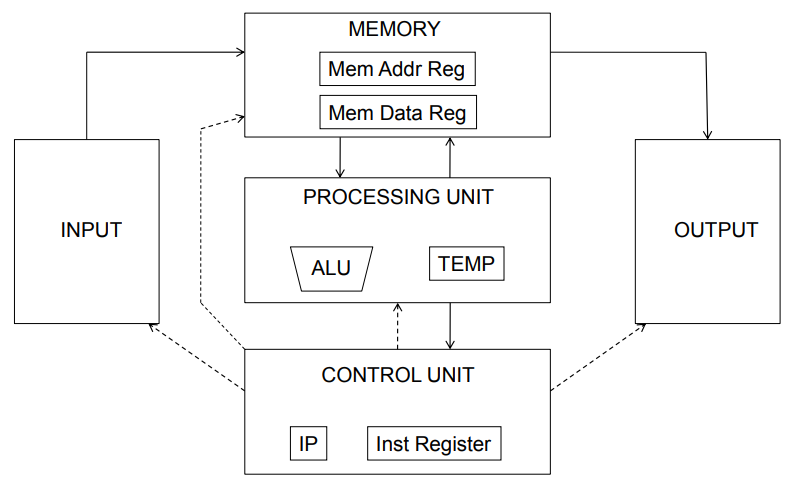
\includegraphics[width=0.4\textwidth]{imagenes/von_neuman_arquichtecture}
	\caption{Arquitectura de Von Newmman}
	\label{fig:vonneumanarquichtecture}
\end{figure}
Cada instrucción, es extraida de la memoria usando la dirección indicada por el \textbf{Instruction Pointer}. La unidad de control se encarga de indicar a la memoria si son necesarios otros valores para poder llevar a cabo la ejecución de la instrucción y luego pasa todo los datos a la unidad de procesamiento.

Sin embargo, la implementación de las ISA (microarquitectura) fue cambiando drásticamente para mejorar el rendimiento de este ciclo.

\section{Microarquitectura}
La micoarquitectura es la implementación a nivel hardware de la ISA, es decir, es un conjunto de componentes electrónicos organizados de cierta manera para que respeten esas especificaciones. En la sección \ref{Intro::ISA::Von_Neuman}, vimos como el usuario ve el ciclo de instrucciones. Desde el punto de vista de la implementación (hardware), el ciclo es realizado por unidades de procesamiento que operan sobre los datos de acuerdo a ciertas señales. 

Cada instrucción es una señal que usa el procesador de instrucciones para decidir que conjunto de componentes electronicos deben ser activados para poder llevar a cabo la operación deseada. Especificamente, las instrucciones indican: 

\begin{itemize}
	\item \textbf{Datapath:} Que elementos deben manejar y transformar los datos (unidades de procesamiento, de almacenamiento y estructuras de hardware que permiten el flujo de datos)
	\item \textbf{Control Logic:} Que elementos de hardware determinan las señales de control que indican al datapath lo que debe hacer con los datos.
\end{itemize}

En este nivel, ocurren muchas \textit{cosas} que no son visibles para el programador y están destinadas a optimizar el tiempo de ejecución de las instruccions. Estas \textit{cosas} pueden ser algoritmos implementado a nivel electrónico o agregado de componentes que permiten acelerar alguna etapa del ciclo. Algunas de las características encontradas en las microarquitecturas actuales son:

\begin{itemize}
	\item Pipelining
	\item Ejecución de múltiple instrucciones simultáneamente.
	\item Ejecución fuera de orden
	\item y Cachés de dato e instrucciones separadas, entre otros.
\end{itemize}

\subsection{Medidas de Performance}
La escala y complejidad de los sistemas de software modernos, junto con las técnicas usadas por los diseñadores de hardware para mejorar el rendimiento de los dispositivos, ha logrado hacer que el rendimiento pueda depender de varios factores.

\subsection{Response time:}
A veces, mediremos el rendimiento de una computadora en base a su tiempo de respuesta (\textbf{response time} o \textbf{execution time}) - el tiempo entre que pasa entre que una tarea empieza y termina -. Este tiempo se mide en segundos por programa y mide el tiempo total que toma completar una tarea, incluyendo accesos a memoria, operaciones del sistema, etc.

En la práctica, la computadora es compartida por varios programas y los microprocesadores deben ejecutar varias tareas simultáneamente. En estos casos, deberemos tener en cuenta que la tarea que la tarea que se está evaluando, no está siendo ejecutada todo el tiempo por lo qué habrá que distinguir el tiempo que el procesador pasa ejecutando la tarea  \textbf{CPU Time} del tiempo en el que está procesando otros programas.

Entonces, el tiempo de ejecución se define de la siguiente manera:

$$Response~Time = \frac{Clock~Cycles~spent~on~task}{Clock~Rate}$$

Donde \textit{Clock Cycle} son la cantidad de ciclos de reloj (ticks) que se utilizaron en la tarea y \textit{Clock Rate} es el tiempo que dura cada tick del reloj.

\nocite{*}
\bibliographystyle{plain}
\bibliography{bibliography}
\end{document}

